\section{天地玄黄}
帝高阳之苗裔兮,朕皇考曰伯庸。
摄提贞于孟陬兮,惟庚寅吾以降。
皇览揆余初度兮,肇锡余以嘉名。
名余曰正则兮,字余曰灵均。
纷吾既有此内美兮,又重之以修能。
扈江离与辟芷兮,纫秋兰以为佩。
汩余若将不及兮,恐年岁之不吾与。
朝搴阰之木兰兮,夕揽洲之宿莽。
日月忽其不淹兮,春与秋其代序。
惟草木之零落兮,恐美人之迟暮。
不抚壮而弃秽兮,何不改乎此度?

\begin{customfigure}{梅开一度}
	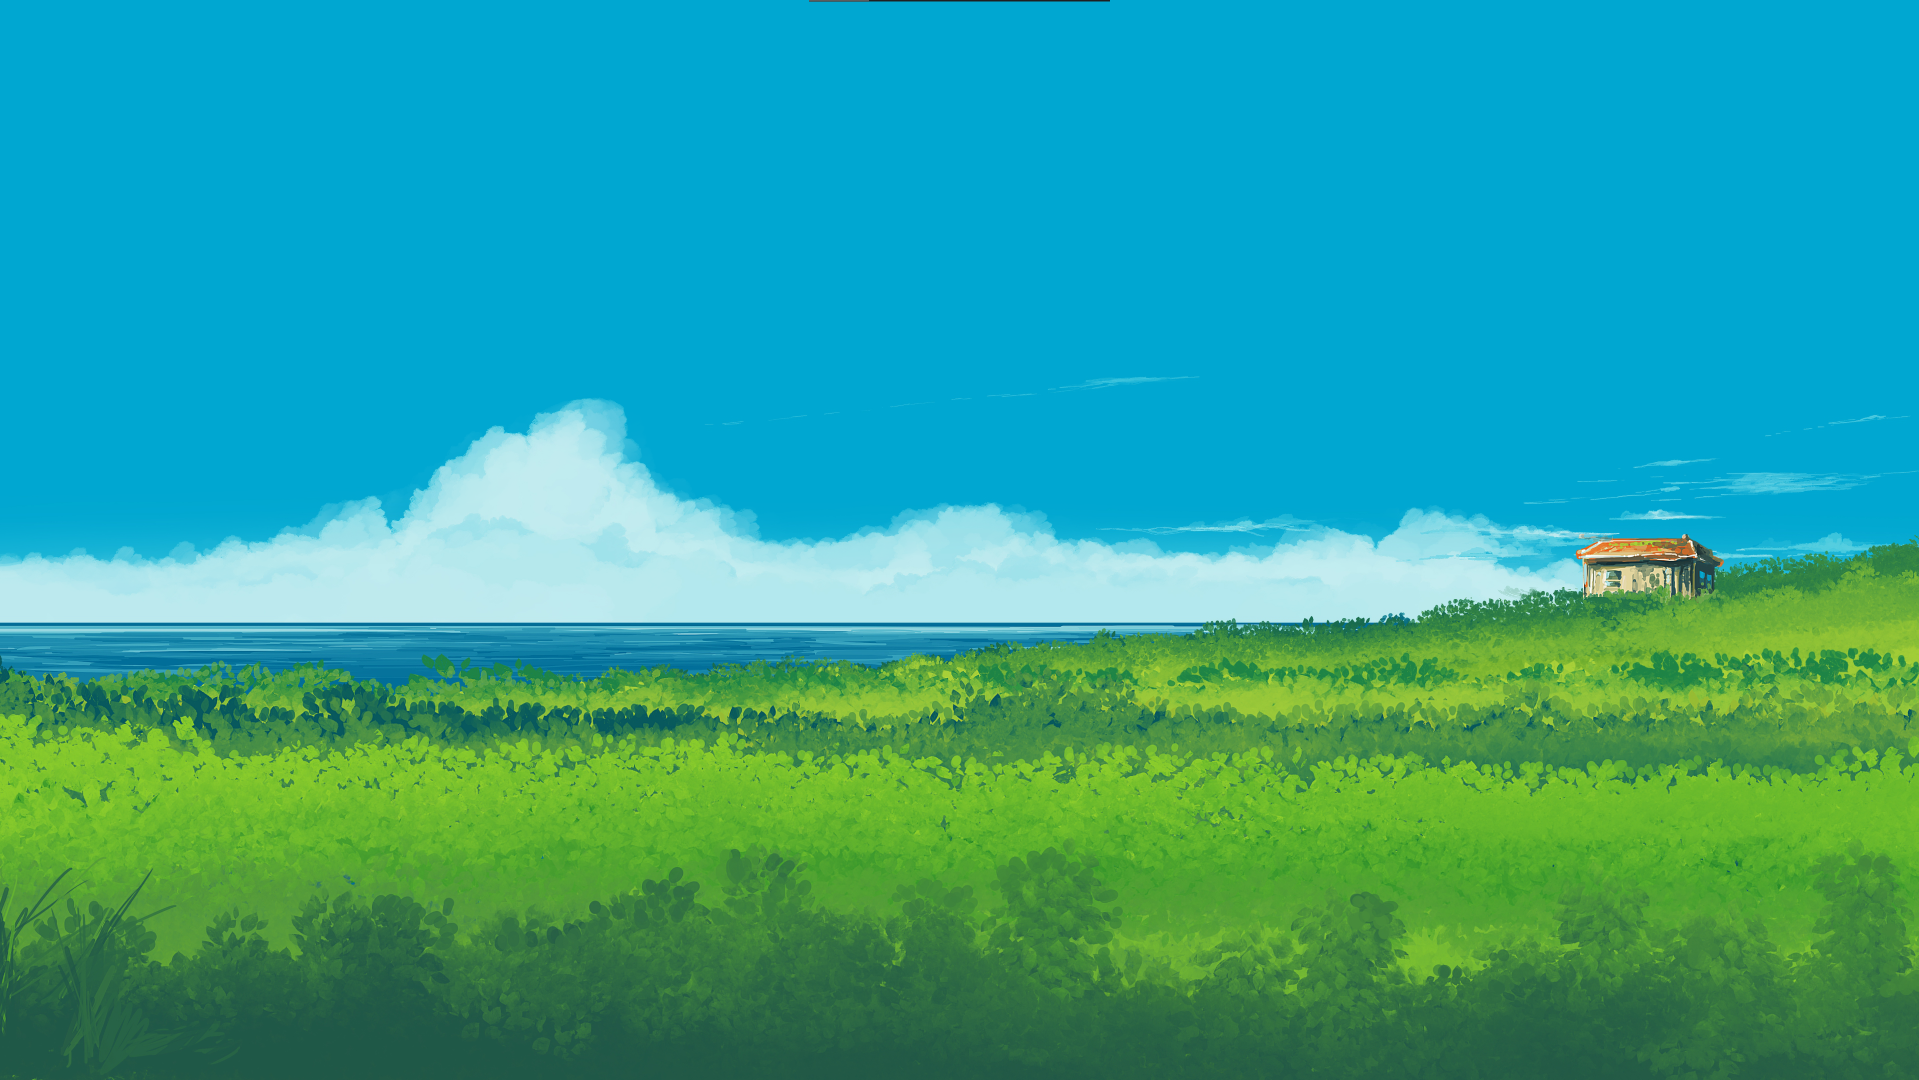
\includegraphics[width=0.8\textwidth]{figures/test2.png} % 你的图片路径
\end{customfigure}

乘骐骥以驰骋兮,来吾道夫先路!
昔三后之纯粹兮,固众芳之所在。
杂申椒与菌桂兮,岂惟纫夫蕙茝!
彼尧舜之耿介兮,既遵道而得路。
何桀纣之猖披兮,夫唯捷径以窘步。
惟夫党人之偷乐兮,路幽昧以险隘。
岂余身之惮殃兮,恐皇舆之败绩!
忽奔走以先后兮,及前王之踵武。
荃不查余之中情兮,反信谗而齌怒。
余固知謇謇之为患兮,忍而不能舍也。
指九天以为正兮,夫唯灵修之故也。
曰黄昏以为期兮,羌中道而改路!
初既与余成言兮,后悔遁而有他。
余既不难夫离别兮,伤灵修之数化。
余既滋兰之九畹兮,又树蕙之百亩。
畦留夷与揭车兮,杂杜衡与芳芷。
冀枝叶之峻茂兮,愿俟时乎吾将刈。
虽萎绝其亦何伤兮,哀众芳之芜秽。
众皆竞进以贪婪兮,凭不厌乎求索。
羌内恕己以量人兮,各兴心而嫉妒。
忽驰骛以追逐兮,非余心之所急。
老冉冉其将至兮,恐修名之不立。
朝饮木兰之坠露兮,夕餐秋菊之落英。
苟余情其信姱以练要兮,长顑颔亦何伤。
掔木根以结茝兮,贯薜荔之落蕊。
矫菌桂以纫蕙兮,索胡绳之纚纚。
謇吾法夫前修兮,非世俗之所服。
虽不周于今之人兮,愿依彭咸之遗则。

长太息以掩涕兮,哀民生之多艰。
余虽好修姱以鞿羁兮,謇朝谇而夕替。
既替余以蕙纕兮,又申之以揽茝。
亦余心之所善兮,虽九死其犹未悔。
怨灵修之浩荡兮,终不察夫民心。
众女嫉余之蛾眉兮,谣诼谓余以善淫。
固时俗之工巧兮,偭规矩而改错。
背绳墨以追曲兮,竞周容以为度。
忳郁邑余侘傺兮,吾独穷困乎此时也。
宁溘死以流亡兮,余不忍为此态也。
鸷鸟之不群兮,自前世而固然。
何方圜之能周兮,夫孰异道而相安?
屈心而抑志兮,忍尤而攘诟。
伏清白以死直兮,固前圣之所厚。
悔相道之不察兮,延伫乎吾将反。
回朕车以复路兮,及行迷之未远。
步余马于兰皋兮,驰椒丘且焉止息。
进不入以离尤兮,退将复修吾初服。
制芰荷以为衣兮,集芙蓉以为裳。
不吾知其亦已兮,苟余情其信芳。
高余冠之岌岌兮,长余佩之陆离。
芳与泽其杂糅兮,唯昭质其犹未亏。
忽反顾以游目兮,将往观乎四荒。
佩缤纷其繁饰兮,芳菲菲其弥章。
民生各有所乐兮,余独好修以为常。
虽体解吾犹未变兮,岂余心之可惩\cite{JiangShuZhen2025,johnke2025,li2025a}。

女媭之婵媛兮,申申其詈予,曰:

鲧婞直以亡身兮,终然夭乎羽之野。
汝何博謇而好修兮,纷独有此姱节?
薋菉葹以盈室兮,判独离而不服。
众不可户说兮,孰云察余之中情?如图~\ref{fig:1-1} 所示。
世并举而好朋兮,夫何茕独而不予听?
依前圣以节中兮,喟凭心而历兹。
济沅湘以南征兮,就重华而陈词:
启《九辩》与《九歌》兮,夏康娱以自纵。
不顾难以图后兮,五子用失乎家衖。
羿淫游以佚畋兮,又好射夫封狐。
固乱流其鲜终兮,浞又贪夫厥家。
浇身被服强圉兮,纵欲而不忍。
日康娱而自忘兮,厥首用夫颠陨。
夏桀之常违兮,乃遂焉而逢殃。
后辛之菹醢兮,殷宗用而不长。
汤禹俨而祗敬兮,周论道而莫差。
举贤才而授能兮,循绳墨而不颇。
皇天无私阿兮,览民德焉错辅。
夫维圣哲以茂行兮,苟得用此下土。
瞻前而顾后兮,相观民之计极。
夫孰非义而可用兮?孰非善而可服?
阽余身而危死兮,览余初其犹未悔。
不量凿而正枘兮,固前修以菹醢。
曾歔欷余郁邑兮,哀朕时之不当。
揽茹蕙以掩涕兮,沾余襟之浪浪。
跪敷衽以陈辞兮,耿吾既得此中正。
驷玉虬以椉鹥兮,溘埃风余上征。\cite{LiuDongLing2025,MaJie2025}
朝发轫于苍梧兮,夕余至乎县圃。
欲少留此灵琐兮,日忽忽其将暮。
吾令羲和弭节兮,望崦嵫而勿迫。
路曼曼其修远兮,吾将上下而求索。
饮余马于咸池兮,总余辔乎扶桑。
折若木以拂日兮,聊逍遥以相羊。
前望舒使先驱兮,后飞廉使奔属。
鸾皇为余先戒兮,雷师告余以未具。
吾令凤鸟飞腾兮,继之以日夜。
飘风屯其相离兮,帅云霓而来御。
纷总总其离合兮,斑陆离其上下。
吾令帝阍开关兮,倚阊阖而望予。
时暧暧其将罢兮,结幽兰而延伫。
世溷浊而不分兮,好蔽美而嫉妒。
朝吾将济于白水兮,登阆风而绁马。
忽反顾以流涕兮,哀高丘之无女。
溘吾游此春宫兮,折琼枝以继佩。
及荣华之未落兮,相下女之可诒。
吾令丰隆乘云兮,求宓妃之所在。\cite{pribyl2025a}
解佩纕以结言兮,吾令謇修以为理。
纷总总其离合兮,忽纬繣其难迁。
夕归次于穷石兮,朝濯发乎洧盘。
保厥美以骄傲兮,日康娱以淫游。
虽信美而无礼兮,来违弃而改求。
览相观于四极兮,周流乎天余乃下。
望瑶台之偃蹇兮,见有娀之佚女。
吾令鸩为媒兮,鸩告余以不好。
雄鸠之鸣逝兮,余犹恶其佻巧。
心犹豫而狐疑兮,欲自适而不可。
凤皇既受诒兮,恐高辛之先我。
欲远集而无所止兮,聊浮游以逍遥。
及少康之未家兮,留有虞之二姚。
理弱而媒拙兮,恐导言之不固。
世溷浊而嫉贤兮,好蔽美而称恶。
闺中既以邃远兮,哲王又不寤。
怀朕情而不发兮,余焉能忍而与此终古?
索琼茅以筳篿兮,命灵氛为余占之。
曰:两美其必合兮,孰信修而慕之?
思九州之博大兮,岂惟是其有女?
曰:勉远逝而无狐疑兮,孰求美而释女?
何所独无芳草兮,尔何怀乎故宇?
世幽昧以昡曜兮,孰云察余之善恶?
民好恶其不同兮,惟此党人其独异!
户服艾以盈要兮,谓幽兰其不可佩。
览察草木其犹未得兮,岂珵美之能当?
苏粪壤以充帏兮,谓申椒其不芳。
欲从灵氛之吉占兮,心犹豫而狐疑。
巫咸将夕降兮,怀椒糈而要之。
百神翳其备降兮,九疑缤其并迎。
皇剡剡其扬灵兮,告余以吉故。
曰:勉升降以上下兮,求矩矱之所同。
汤禹俨而求合兮,挚咎繇而能调。
苟中情其好修兮,又何必用夫行媒?
说操筑于傅岩兮,武丁用而不疑。
吕望之鼓刀兮,遭周文而得举。
宁戚之讴歌兮,齐桓闻以该辅。
及年岁之未晏兮,时亦犹其未央。
恐鹈鴂之先鸣兮,使夫百草为之不芳。
何琼佩之偃蹇兮,众薆然而蔽之。
惟此党人之不谅兮,恐嫉妒而折之。
时缤纷其变易兮,又何可以淹留?
兰芷变而不芳兮,荃蕙化而为茅。
何昔日之芳草兮,今直为此萧艾也?
岂其有他故兮,莫好修之害也!
余以兰为可恃兮,羌无实而容长。
委厥美以从俗兮,苟得列乎众芳。
椒专佞以慢慆兮,樧又欲充夫佩帏。
既干进而务入兮,又何芳之能祗?
固时俗之流从兮,又孰能无变化?
览椒兰其若兹兮,又况揭车与江离?
惟兹佩之可贵兮,委厥美而历兹。
芳菲菲而难亏兮,芬至今犹未沬。
和调度以自娱兮,聊浮游而求女。
及余饰之方壮兮,周流观乎上下。
灵氛既告余以吉占兮,历吉日乎吾将行。
折琼枝以为羞兮,精琼爢以为粻。
为余驾飞龙兮,杂瑶象以为车。
何离心之可同兮?吾将远逝以自疏。
邅吾道夫昆仑兮,路修远以周流。
扬云霓之晻蔼兮,鸣玉鸾之啾啾。
朝发轫于天津兮,夕余至乎西极。
凤皇翼其承旗兮,高翱翔之翼翼。
忽吾行此流沙兮,遵赤水而容与。
麾蛟龙使梁津兮,诏西皇使涉予。
路修远以多艰兮,腾众车使径待。
路不周以左转兮,指西海以为期。
屯余车其千乘兮,齐玉轪而并驰。
驾八龙之婉婉兮,载云旗之委蛇。
抑志而弭节兮,神高驰之邈邈。
奏《九歌》而舞《韶》兮,聊假日以媮乐。
陟升皇之赫戏兮,忽临睨夫旧乡。
仆夫悲余马怀兮,蜷局顾而不行。
乱曰:已矣哉!
国无人莫我知兮,又何怀乎故都!
既莫足与为美政兮,吾将从彭咸之所居!